\documentclass{article}
\usepackage[utf8]{inputenc}
\usepackage{amsmath}
\usepackage{amssymb}
\usepackage{amsthm}
\usepackage{stmaryrd}
\usepackage{graphicx}
\usepackage{csquotes}
\usepackage{tikz}
\usetikzlibrary{automata, positioning}
\usepackage{hyperref}
\usepackage{mathtools}
\hypersetup{
    colorlinks=true,
    linkcolor=blue,
    filecolor=magenta,      
    urlcolor=blue,
    citecolor=blue,
    pdfborder={0 0 0} % Removes the red boxes around links
}
\usepackage{extarrows} % For extended arrows
\usepackage{listings}
\usepackage{tikz}
\usetikzlibrary{automata, positioning, arrows.meta, shapes, arrows}
% For better listings
\usepackage{listings}
% For mathbb, mathcal, etc.
\usepackage{amsfonts}
% For clever referencing (optional, but useful)
\usepackage{cleveref}
\usepackage{lmodern,amsmath,amssymb}
%for lowercase calligraphic math
\usepackage{boondox-cal}%for lowercase \mathcal
\usetikzlibrary{arrows.meta,positioning,calc}
\usetikzlibrary{decorations.pathmorphing}
\tikzset{
  state/.style={draw,rectangle,minimum size=2.5mm,inner sep=0pt},
  circ/.style={draw,circle,minimum size=1.5mm,inner sep=0pt, fill=black},
trig/.style={draw,regular polygon,regular polygon sides=3,shape border rotate=180,minimum size=2.5mm,inner sep=0pt},
  hub/.style={state,dashed},
  arr/.style={-{Latex[length=1.6mm]},line width=0.4pt},
  lab/.style={font=\scriptsize,inner sep=1pt,fill=white,fill opacity=.9,text opacity=1},
  ruletitle/.style={font=\bfseries\scriptsize}
}
\usepackage{scalerel}



% Raccourcis type [A]

\newcommand{\quotient}[1]{\llbracket#1\rrbracket}          % creux




\newtheorem{definition}{Definition}[section]
\newtheorem{lemma}[definition]{Lemma}
\newtheorem{proposition}[definition]{Proposition}
\newtheorem{theorem}[definition]{Theorem}
\newtheorem{claim}[definition]{Claim}
\newtheorem{corollary}[definition]{Corollary}
\newtheorem{remark}[definition]{Remark}
\newtheorem{example}[definition]{Example}

\newcommand{\A}{\mathcal{A}}
\newcommand{\B}{\mathcal{B}}
\newcommand{\norm}[1]{| #1 |}
\newcommand{\milner}[1]{\mathcal{M}(#1)}
\newcommand{\normalForm}[1]{\mathcal{N}(#1)}


\definecolor{darkred}{rgb}{0.85, 0.1, 0.2}
\definecolor{darkblue}{rgb}{0.2, 0.2, 0.75}
\definecolor{darkgreen}{rgb}{0.2, 0.6, 0.2}


\begin{document}
\title{Chart semantics for regular expressions:\\characterization and axiomatization}
\author{Your Name}
\date{\today}
\maketitle  
\begin{abstract}
We introduce Milner charts, a class of transition structures naturally associated with regular expressions. Our main contributions are: (i) a rewriting-based characterization that identifies Milner charts among all charts, and (ii) a completeness result establishing that bisimilarity of expressions coincides with their provable equivalence in Milner's equational axiomatization. 
\end{abstract}
\section{Introduction}

\section{Preliminaries}

This section introduces the main concepts used throughout the paper: regular expressions and their chart-based semantics, bisimulation equivalence between charts, and Milner's equational proof system for reasoning about expression equivalence.

\subsection{Regular Expressions}
\begin{definition}
The set of \emph{regular expressions} over an alphabet $\Sigma$ is defined by the following grammar:
\[
e ::= 0 \mid 1 \mid a \mid e + e \mid e\cdot e \mid e^* \qquad (a \in \Sigma)
\]
\end{definition}

\vspace{1em}
\theoremstyle{definition}
\newtheorem{notation}[definition]{Notation}

\begin{notation} 
We sometimes write $ef$ for $e \cdot f$. The precedence of operations is as usual: star, then concatenation, then union. For instance, $e+f^*g$ means $e+(f^*\cdot g)$.
\end{notation}
\vspace{1em}

While the semantics of regular expressions are traditionally defined as word languages, in this paper we will define them through charts, which we introduce in the following section.

\subsection{Charts}
\begin{definition} 
A \emph{chart} over an alphabet $\Sigma$ is a tuple $(Q, \Sigma, \Delta, I, F)$ where:
\begin{itemize}
    \item $Q$ is a finite set of \emph{states},
    \item $\Sigma$ is a finite input alphabet,
    \item $\Delta \subseteq Q \times \Sigma \times Q$ is a set of \emph{transitions},
    \item $I \in Q$ is the \emph{initial} state,
    \item $F \subseteq Q$ is the set of \emph{final} states.
\end{itemize}
The set of derivatives  of a state $q$ is defined by:
\[
D(q)=\{(a,q')\mid(q,a,q')\in\Delta\},
\]
and its finality is the function $\chi$ defined as follows:
\[
\chi(q)=
\begin{cases}
1 & \text{if $q$ is final},\\
0 & \text{otherwise.}
\end{cases}
\]
\end{definition}



\begin{remark}
When clear from context or irrelevant, we omit the alphabet of a chart.
We sometimes define a chart by specifying the derivatives of its states rather than its 
transitions set; this is equivalent. As usual, we shall not distinguish between isomorphic charts. 
\end{remark}

\subsection{Milner Charts}




\begin{definition}
The \emph{union} of two charts $C$ and $D$, denoted $C + D$, 
is obtained by taking their disjoint union, adding a fresh initial state~$s$ 
that inherits the derivatives of the initial states of~$C$ and~$D$, 
and making~$s$ final whenever one of them is final.
Finally, states not reachable from~$s$ are removed.
\end{definition}


\begin{example}  Here is an example of the sum of two charts $C$ and $D$:
  \begin{center}
  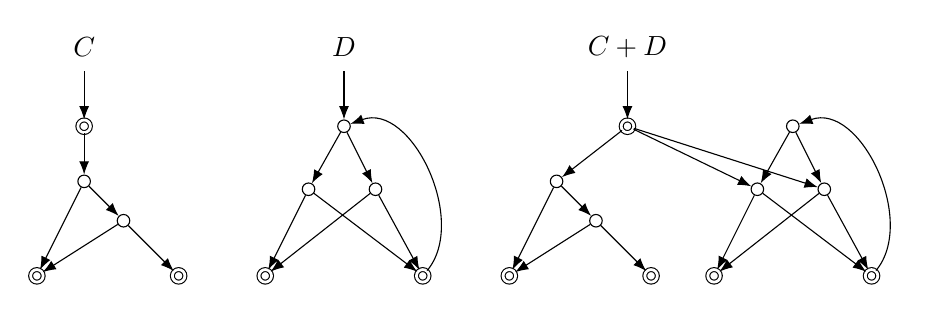
\begin{tikzpicture}[
  >=Latex,
  box/.style={rounded corners, draw, thick, inner sep=8pt, minimum width=2.3cm, minimum height=3cm},
  state/.style={circle, draw, inner sep=1.6pt},
  ghost/.style={circle, draw, inner sep=1.2pt, gray!60},
  final/.style={state, double, double distance=1pt},
  lab/.style={font=\small}
]

%------------ Boîte 1 (C1) -----------------
%\node[box] (B1) at (0,0) {};

% états (vertical compact)
\node (label) at (0,2) {$C$};
\node[final, label={[lab]left:$ $}] (i1) at (0,1.0) {};
\node[state] (q11) at (0,0.3) {};
\node[state] (q12) at (0.5,-0.2) {};
\node[final, label={[lab]below:$ $}]  (f11) at (-0.6,-0.9) {};
\node[final, label={[lab]below:$ $}] (f12) at (1.2,-0.9) {};

% transitions abstraites (patron 1)
\draw[->] (0,1.7) -- (i1.north);
%\draw[->] (i1) -- (q11);
\draw[->] (i1) -- node[lab,right,pos=0.45] {$ $} (q11);
\draw[->] (q11) to (q12);
\draw[->] (q12) -- (f11);
\draw[->] (q12) -- (f12);
\draw[->] (q11) to (f11);

\begin{scope}[shift={(-.7,0)}]

\node[state, label={[lab]left:$ $}] (i2) at (4,1.0) {};
\node[state] (p21) at (3.55,0.2) {};
\node[state] (p22) at (4.4,0.2) {};
\node[final, label={[lab]below:$ $}]  (f21) at (3,-0.9) {};
\node[final, label={[lab]below:$ $}] (f22) at (5,-0.9) {};

\node (label) at (4,2) {$D$};
% transitions abstraites (patron 2)

\draw[->] (4,1.7) -- (i2.north);
\draw[->] (i2) -- node[lab,left,pos=0.45] {$ $} (p21);
\draw[->] (i2) -- node[lab,right,pos=0.45] {$ $} (p22);
\draw[->] (p21) -- (f21);
\draw[->] (p22) -- (f22);
\draw[->] (p21) to (f22);
\draw[->] (p22) to (f21);
\draw[->] (f22) to[in = 20, out=50]  (i2);
\end{scope}
\begin{scope}[shift={(5,0)}]

%------------ Boîte 1 (C1) -----------------
%\node[box] (B1) at (0,0) {};

% états (vertical compact)
%\node[final, label={[lab]above:$ $}] (i1) at (0,1.0) {};

\begin{scope}[shift={(1,0)}]
\node[state] (q11a) at (0,0.3) {};
\node[state] (q12a) at (0.5,-0.2) {};
\node[final, label={[lab]below:$ $}]  (f11a) at (-0.6,-0.9) {};
\node[final, label={[lab]below:$ $}] (f12a) at (1.2,-0.9) {};

% transitions abstraites (patron 1)
%\draw[->] (i1) -- (q11);
\draw[->] (q11a) to (q12a);
\draw[->] (q12a) -- (f11a);
\draw[->] (q12a) -- (f12a);
\draw[->] (q11a) to (f11a);
\end{scope}
%------------ Boîte 2 (C2) -----------------
%\node[box] (B2) at (6,0) {};

% états
\node[state, label={[lab]above:$ $}] (i2a) at (4,1.0) {};
\node[state] (p21a) at (3.55,0.2) {};
\node[state] (p22a) at (4.4,0.2) {};
\node[final, label={[lab]below:$ $}]  (f21a) at (3,-0.9) {};
\node[final, label={[lab]below:$ $}] (f22a) at (5,-0.9) {};


% transitions abstraites (patron 2)
\draw[->] (i2a) -- (p21a);
\draw[->] (i2a) -- (p22a);
\draw[->] (p21a) -- (f21a);
\draw[->] (p22a) -- (f22a);
\draw[->] (p21a) to (f22a);
\draw[->] (p22a) to (f21a);
\draw[->] (f22a) to[in = 20, out=50] (i2a);

%------------ Nouvel état initial i (somme) --------------
\node (label) at (1.9,2) {$C + D$};
\node[final, label={[lab]right:$ $}] (inew) at (1.9,1.0) {}; % final car i1 est final
% flèche initiale globale
\draw[->] (1.9,1.7) -- (inew.north);

% Transitions de i vers les cibles des transitions de i1 et i2
% (elles reproduisent: (i,a,q) si (i1,a,q) ou (i2,a,q) étaient dans Δ1 ou Δ2)
\draw[->] (inew) -- node[lab,above,pos=0.55] {$ $} (q11a);
%\draw[->] (inew) -- node[lab,above,pos=0.55] {$b$} (q12);
\draw[->] (inew) -- node[lab,below,pos=0.45] {$ $} (p21a);
\draw[->] (inew) -- node[lab,above,pos=0.45] {$ $} (p22a);

\end{scope}

\end{tikzpicture}
\end{center}
\end{example}




\begin{definition}
The \emph{sequential composition} of two charts $C$ and $D$, denoted $C \cdot D$, 
is obtained from their disjoint union by adding to the derivatives of each final state of~$C$ 
the derivatives of the initial state of~$D$, and marking it final 
whenever the initial state of~$D$ is final. 
The initial state of~$C$ becomes that of the composition, 
and unreachable states are removed.
\end{definition}

\begin{example} An example of sequential composition of two charts $C$ and $D$:
    \begin{center}
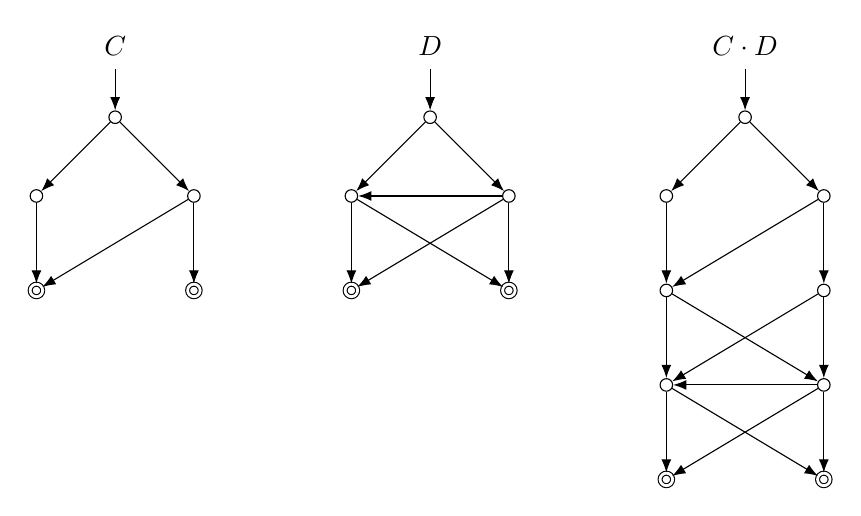
\begin{tikzpicture}[
  >=Latex,
  state/.style={circle, draw, inner sep=1.6pt},
  ghost/.style={circle, draw, inner sep=1.2pt, gray!60},
  final/.style={state, double, double distance=1pt},
  lab/.style={font=\small},
  every edge quotes/.style={auto, text=black, font=\small}
]

% ======================= C1 (gauche->droite) =======================
\begin{scope}[shift={(-6,0)},rotate=-90]
  \node (labC1) at (-2.1,0) {$C$};

  % états C1
  \node[state] (i1) at (-1.2,0) {};
  \node[state] (x1) at (-0.2,1) {};
  \node[state] (x2) at (-0.2,-1) {};
  \node[final] (f1) at (1.0,1) {};
  \node[final] (f1p) at (1.0,-1) {};

  % flèche initiale
  \draw[->] ([xshift=-15pt]i1.north) -- (i1.north);

  % transitions internes (gris)
  \draw[->] (i1) -- (x1);
  \draw[->] (i1) -- (x2);
  \draw[->] (x1) -- (f1);
  \draw[->] (x2) -- (f1p);
  \draw[->] (x1) to (f1p);
\end{scope}

% ======================= C2 (gauche->droite) =======================
\begin{scope}[shift={(-2,0)}, ,rotate=-90]
  \node (labC2) at (-2.1,0) {$D$};

  % états C2
  \node[state] (i2) at (-1.2,0) {};
  \node[state] (y1) at (-0.2,1) {};
  \node[state] (y2) at (-0.2,-1) {};
  \node[final] (g1) at (1.0,1) {};
  \node[final] (g2) at (1.0,-1) {};

  % flèche initiale
  \draw[->] ([xshift=-15pt]i2.north) -- (i2.north);

  % sorties explicites de i2
  \draw[->] (i2) -- (y1) node[midway,above,lab] {$ $};
  \draw[->] (i2) -- (y2) node[midway,below,lab] {$ $};

  % transitions internes (gris)
   \draw[->] (y1) -- (y2);
  \draw[->] (y1) -- (g1);
  \draw[->] (y2) -- (g2);
  \draw[->] (y1) to (g2);
  \draw[->] (y2) to (g1);
\end{scope}
\begin{scope}[shift={(2,0)}, rotate=-90]
    \node (labSeq) at (-2.1,0) {$C \cdot D$};

% copie visuelle de C1 (à gauche)
\node[state] (i1s) at (-1.2,0) {};
\node[state] (xs1) at (-0.2,1) {};
\node[state] (xs2) at (-0.2,-1) {};
\node[state] (fs1) at (1.0,1) {};
\node[state] (fs2) at (1.0,-1) {};


% copie visuelle de C2 (à droite)
%\node[state] (i2s) at (1.0,0) {}; % i2 lui-même n'est pas final
\node[state] (ys1) at (2.2,1) {};
\node[state] (ys2) at (2.2,-1) {};
\node[final] (gs1) at (3.4,1) {};
\node[final] (gs2) at (3.4,-1) {};

% flèche initiale globale: i1
\draw[->] ([xshift=-15pt]i1s.north) -- (i1s.north);

% Δ1 (gris)
\draw[->] (i1s) -- (xs1);
\draw[->] (i1s) -- (xs2);
\draw[->] (xs1) -- (fs1);
\draw[->] (xs2) -- (fs2);
\draw[->] (xs1) to (fs2);

% Δ2 (gris)
%\draw[->, dashed] (i2s) -- (ys1);
%\draw[ ->, double] (i2s) -- (ys2);
\draw[->] (ys1) -- (gs1);
\draw[->] (ys1) -- (ys2);
\draw[->] (ys2) -- (gs2);
\draw[->] (ys1) to (gs2);
\draw[->] (ys2) to (gs1);

% Règle de concaténation: copier sorties de i2 sur chaque f∈F1
% Utilisation de bend pour éviter croisements
\draw[->] (fs1) to[bend left=0] node[lab,above] {$ $} (ys1);
\draw[->] (fs1) to[bend left=0] node[lab,below] {$ $} (ys2);

\draw[->] (fs2) to[bend right=0] node[lab,below] {$ $} (ys1);
\draw[->] (fs2) to[bend right=0] node[lab,above] {$ $} (ys2);

\end{scope}
\end{tikzpicture}
\end{center}
\end{example}

\begin{definition}
The \emph{Kleene star} of a chart $C$, denoted $C^*$, 
is obtained by adding to each final state of~$C$ 
the derivatives of its initial state, 
which remains initial and becomes also final. 
Unreachable states are then removed.
\end{definition}


\begin{example} Example of a chart iteration. 
\begin{center}
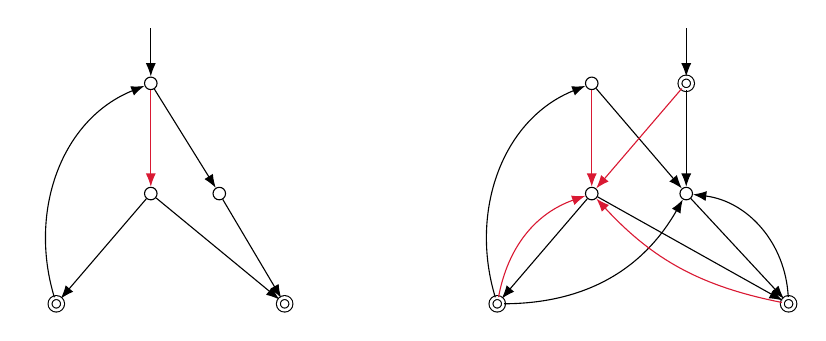
\begin{tikzpicture}[
  >=Latex,
  state/.style={circle, draw, inner sep=1.6pt},
  ghost/.style={circle, draw, inner sep=1.2pt, gray!60},
  final/.style={state, double, double distance=1pt},
  lab/.style={font=\small},
  every edge quotes/.style={auto, text=black, font=\small}
]

% ======================= C (vertical) =======================
\begin{scope}[shift={(-2.8,0)}]
  %\node (labC) at (0,2.3) {$C$};

  % états C
  \node[state] (i1) at (0,1.4) {};
  \node[state] (q1) at (0,-0) {};
  \node[state] (q2) at ( 0.87,-0) {};
  \node[final] (f1) at (-1.2,-1.4) {};
  \node[final] (f2) at ( 1.7,-1.4) {};

  % flèche initiale
  \draw[->] (0,2.1) -- (i1.north);

  % sorties explicites de i1
  \draw[->, darkred] (i1) -- (q1);
  \draw[ ->] (i1) -- (q2);

  % transitions internes (gris)
  \draw[->] (q1) to (f1);
  \draw[->] (q2) to (f2);
  \draw[->] (q1) to (f2);
  \draw[->] (f1) to[bend left, in=135, out =40]  (i1);
\end{scope}

% ======================= C* (vertical) =======================
\begin{scope}[shift={(2.8,0)}]
  %\node (labS) at (0,2.8) {$C^{\!*}$};

  % nouvel initial i (final aussi)
  \node[final] (i)  at (1.2,1.4) {};

    \node[state] (i1s) at (0,1.4) {};
  \node[state] (r1) at (0,-0) {};
  \node[state] (r2) at ( 1.2,-0) {};
  \node[final] (g1) at (-1.2,-1.4) {};
  \node[final] (g2) at ( 2.5,-1.4) {};



  % flèche initiale globale
  \draw[->] (1.2,2.1) -- (i.north);

  % Δ (gris) : transitions internes de C conservées
  \draw[->,darkred] (i1s) -- (r1);
  \draw[->] (i1s) -- (r2);
    \draw[darkred, ->] (i) -- (r1);
  \draw[->] (i) -- (r2);
  \draw[->] (r1)  to (g1);
  \draw[->] (r2)  to  (g2);
  \draw[->] (r1)  to  (g2);
  \draw[->] (g1)  to[bend left, in=135, out =40]  (i1s);
  % Ajouts pour l'étoile :
  % 1) Depuis i, recopier les sorties de i1
 % \draw[->] (i) to node[midway,above,lab] {$ $} (r1);
  %\draw[->,darkred] (i) to node[midway,above,lab] {$$} (r2);

  % 2) Depuis chaque f \in F, recopier les sorties de i1 (itération)
  %    ici F = {g1, g2}
  \draw[->,darkred ] (g1) to[bend left=30]  node[midway,left,lab]  {$ $} (r1);
\draw[->] (g1) to[bend right=30] node[midway,above,lab] {$ $} (r2);


\draw[->,darkred]
    (g2) to[bend left=18] node[midway,right,lab] {$ $} (r1);
\draw[->]
    (g2) to[bend right=40] node[midway,above,lab] {$ $} (r2);
\end{scope}

\end{tikzpicture}
\end{center}
\end{example}


\begin{definition}
The constant chart $\mathbf{0}$ has a single state, which is initial and non-final, with no transitions.  
The constant chart $\mathbf{1}$ has a single state, both initial and final, with no transitions.  
For each letter $a$, the chart $\mathbf{a}$ has two states, one initial and one final, 
connected by a single $a$-labeled transition.
\end{definition}

\begin{definition}
The \emph{Milner chart} of an expression~$e$ over the alphabet $\Sigma$, denoted $M(e)$, is defined by induction as follows, 
where  $a \in \Sigma$:
\[
\begin{array}{rclcrclcrcl}
\milner{0} &\hspace{-8pt}=\hspace{-8pt}& \mathbf{0} & &
\milner{1} &\hspace{-8pt}=\hspace{-8pt}& \mathbf{1} &  &
\milner{a} &\hspace{-8pt}=\hspace{-8pt}& \mathbf{a} \\[4pt]
\milner{e+f} &\hspace{-8pt}=\hspace{-8pt}& \milner{e}+\milner{f} & &
\milner{e\cdot f} &\hspace{-8pt}=\hspace{-8pt}& \milner{e}\cdot\milner{f} & &
\milner{e^*} &\hspace{-8pt}=\hspace{-8pt}& \milner{e}^*
\end{array}
\]
\end{definition}

\begin{example} The milner chart of $a(b+c), (a(b+c))^*$ et $ab^*+c^*$.
\end{example}


\begin{definition} A chart is \emph{rooted} if its initial state has no ingoing transitions.
\end{definition}

\begin{proposition}
For every regular expression $e$, $\milner{e}$ is rooted.
\end{proposition}

\subsection{Bisimulation}
\begin{notation}
    If $C$ is a chart, we denote by $\xlongrightarrow{a}_{C}$ the relation on its set of states defined as:
    $$\xlongrightarrow{a}_{C} \;=\; \{ (p,q) \mid (p,a,q) \text{ is a transition of } C \}.$$
    We denote by $\xlongleftarrow{a}_{C}$ the converse of $\xlongrightarrow{a}_{C}$.
\end{notation}

\begin{definition}
Let $C$ and $D$ be two charts with state sets $Q$ and $Q'$ and respectively. A relation $R\subseteq Q\times Q'$ is a \emph{bisimulation} between $C$ and $D$ if:
\begin{itemize}
    \item $(p,q)\in R \ \ \Rightarrow\ \ \chi(p)=\chi(q)$, 
    \item $\xlongleftarrow{a}_{C}\cdot R\ =\ R \cdot \xlongleftarrow{a}_{D}$ and
    \item $\xlongrightarrow{a}_{C} \cdot R\ =\ R \cdot \xlongrightarrow{a}_{D}$.
\end{itemize}

Let $(p,q)\in C\times D$. We say that $p$ and $q$ are \emph{bisimilar}, and write $p\sim q$, if $(p,q)\in R$ for some bisimilation $R$ between $C$  and $D$.\\

We say that $C$ and $D$ are \emph{bisimilar}, and write $C \sim D$, if there initial states are bisimilar.
\end{definition}

\subsection{Milner's Axiomatization}


\begin{definition} For every expression $e$, we say that $e$ is \emph{final}, and write $e\Downarrow$, if the initial state of $\milner{e}$ is final. We write $e\Uparrow$ otherwise.
    \end{definition}




\begin{definition} \emph{Milner's proof system} 
    contains the following axioms and deduction rules:~\\
    
\textbf{Algebraic laws:}
\[
\renewcommand{\arraystretch}{1.6} % espace vertical entre lignes
\begin{array}{@{\hspace{3pt}}r@{\hspace{6pt}}l
                  @{\hspace{25pt}}r@{\hspace{6pt}}l
                  @{\hspace{25pt}}r@{\hspace{6pt}}l}
\text{\scriptsize (1)}  & e + f = f + e            
  & \text{\scriptsize (5)}  & (ef)g = e(fg)         
  & \text{\scriptsize (9)}  & e + 0 = e \\

\text{\scriptsize (2)}  & (e + f) + g = e + (f + g) 
  & \text{\scriptsize (6)}  & 1e = e = e1           
  & \text{\scriptsize (10)} & 0e = 0 = e0 \\

\text{\scriptsize (3)}  & e + e = e                 
  & \text{\scriptsize (7)}  & (e+f)g = eg + fg      
  & \text{\scriptsize (11)} & 0^* = 1 \\

\text{\scriptsize (4)}  & e^* = 1 + e e^*           
  & \text{\scriptsize (8)}  & e^* = (e+1)^*         
  &                     & 
\end{array}
\]

\textbf{Salooma's induction rule:}
\vspace{.5em}
\[
\frac{\, f= ef + g\qquad e\Uparrow\,}{\,f=e^*g\,}
\]

\textbf{Congruence rules:}
\[
\renewcommand{\arraystretch}{1.8}
\begin{array}{c@{\hspace{35pt}}c@{\hspace{35pt}}c}
\dfrac{}{\,e = e\,} 
  & \dfrac{\,e = f\,}{\,f = e\,} 
  & \dfrac{\,e = f \;\; f = h\,}{\,e = h\,} \\[12pt]
\dfrac{\,e_1 = f_1 \;\; e_2 = f_2\,}{\,e_1 + e_2 = f_1 + f_2\,}
  & \dfrac{\,e_1 = f_1 \;\; e_2 = f_2\,}{\,e_1 e_2 = f_1 e_2\,}
  & \dfrac{\,e = f\,}{\,e^{*} = f^{*}\,}
\end{array}
\]
\vspace{1em}

We say that two regular expressions $e$ and $f$ are \emph{provably equivalent} in the Milner system, denoted $e \equiv f$, if the equation $e = f$ is derivable from the axioms (1-11), Salomaa's  rule and congruence rules.
\end{definition}


Our goal in the remainder of this paper is to address two questions:  
whether Milner charts can be recognized among all charts,  
and whether Milner’s axiomatization is complete with respect to bisimulation equivalence.  
We will answer these questions by means of a rewriting system introduced in the next section.

\section{Rewriting system for charts}

We work with a slightly broader class of structures,  
called \emph{networks}, which extend ordinary charts by allowing multiple inputs.  
The rewriting system will be defined on these networks.

\begin{definition}
  A \emph{network} has the same data as a chart, but instead of a single initial state, it has a set of initial states.
\end{definition}

\begin{definition} We consider the rewriting rules of Figure~\ref{fig:rewriting-rules}, 
which transform networks over~$\Sigma^*$ into networks over~$\Sigma^*$. 
In this picture,
\begin{itemize}
    \item squares denote states for which only some transitions are shown,
    \item circles denote states whose transitions are all explicitly displayed,
    \item circles are distinct from surrounding nodes and are neither initial nor final.
\end{itemize}
We write~$\twoheadrightarrow$ for the union of all these rewriting rules.\end{definition}
                    
                    \begin{figure}[h!]
                      \begin{center} 
                      %  \fboxsep=10pt  % padding between content and box
%\fboxrule=1pt   \fbox{%
\begin{tabular}{ccc}
\textbf{Zero} & \quad & \textbf{Parallel merge} \\[20pt]
  \begin{tikzpicture}[node distance=1.8cm, scale=1.0, every node/.style={transform shape}]
            % Left side (before)
            \node[state] (p1) at (0,0) {};
            \node[state] (q1) at (0,-1.8) {};      
            % Arrow between rules
            \node (i) at (1.5,-0.9) {$\twoheadrightarrow_{\mathsf{0}}$};
            %\node[below=1.2cm of i] {Zero rule};
            % Right side (after)
            \node[state] (p2) at (3,0) {};
            \node[state] (q2) at (3,-1.8) {};
            \draw[arr] (p2) to node[right] {$0$} (q2);  
        \end{tikzpicture} &  \quad &\begin{tikzpicture}[node distance=1.8cm, scale=1.0, every node/.style={transform shape}]
            % Left side (before)
            \node[state] (p1) at (0,0) {};
            \node[state] (q1) at (0,-1.8) {};
            \draw[arr] (p1) to[bend left=20] node[right] {$f$} (q1);
            \draw[arr] (p1) to[bend right=20] node[left]  {$e$} (q1);

            % Arrow between rules
            \node (i) at (1.5,-0.9) {$\twoheadrightarrow_{\mathsf{p}}$};
           % \node[below=1.2cm of i] {Transitions fusion};
        
            % Right side (after)
            \node[state] (p2) at (3,0) {};
            \node[state] (q2) at (3,-1.8) {};
            \draw[arr] (p2) to node[right] {$e+f$} (q2);
        \end{tikzpicture}\\[25pt]
  \textbf{State elimination}  &  & \textbf{Renaming} \\[20pt]
  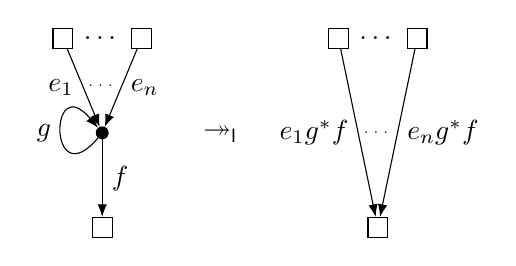
\begin{tikzpicture}[node distance=1.8cm, scale=1.0, every node/.style={transform shape}]
            % Left side (before)
            \node[state] (p1) at (6,0) {};
            \node (d1) at (6.5,0) {$\dots$};
            \node[state] (q1) at (7,0) {};
            \node[circ] (r1) at (6.5,-1.2) {};
            \node[state] (s1) at (6.5,-2.4) {};
            \draw[arr] (p1) to node[left] {$e_1$} (r1);
            \draw[arr] (q1) to node[right] {$e_n$} (r1);
            \draw[arr] (r1) to node[right] {$f$} (s1);
            \draw[arr] (r1) to[loop left, looseness=20, out=-130, in=130] node[left] {$g$} (r1);
            \node (d1') at (6.5,-.6) {\tiny $\dots$};
            % Arrow between rules
            \node (i) at (8,-1.2) {$\twoheadrightarrow_\mathsf{l}$};
            %\node[below=2cm of i] {Safe loop elimination ($g\Uparrow$ only)};

            % Right side (after)
            \pgfmathsetmacro{\shift}{9.5}
            \node[state] (p2) at (\shift,0) {};
            \node[state] (q2) at (\shift+1,0) {};
            \node[state] (s2) at (\shift+0.5,-2.4) {};
            \draw[arr] (p2) to node[left] {$e_1g^*f$} (s2);
            \draw[arr] (q2) to node[right] {$e_ng^*f$} (s2);
            \node (d2) at (\shift+0.5,0) {$\dots$};
            \node (d2') at (\shift+0.5,-1.2) {{\tiny $\dots$}};
        \end{tikzpicture}&&     \begin{tikzpicture}[node distance=1.8cm, scale=1.0, every node/.style={transform shape}]
            % Left side (before)
            \node[state] (p1) at (0,0) {};
            \node[state] (q1) at (0,-1.8) {};  

            \draw[arr] (p1) to node[right] {$e$} (q1);
            % Arrow between rules
            \node (i) at (1.5,-0.9) {$\twoheadrightarrow_{\mathsf{r}}$};
            %\node[below=1.2cm of i] {Renaming};
            % Right side (after)
            \node[state] (p2) at (3,0) {};
            \node[state] (q2) at (3,-1.8) {};
            \draw[arr] (p2) to node[right] {$f$} (q2);  
        \end{tikzpicture}\\[25pt]
          \textbf{Unproductivity elimination}  & &\textbf{Factorization} \\[20pt]
            \begin{tikzpicture}[node distance=1.8cm, scale=1.0, every node/.style={transform shape}]
            % Left side (before)
            \node[circ] (p1) at (0,0) {};
            \node[state] (q1) at (0,-1.8) {};   
            \draw[arr] (p1) to node[right] {$e$} (q1);
            % Arrow between rules
            \node (i) at (1.5,-0.9) {$\twoheadrightarrow_{\mathsf{u}}$};
            %\node[below=1.2cm of i] {Zero rule};
            % Right side (after)
            \node[state] (q2) at (3,-1.8) {};
        \end{tikzpicture}&&           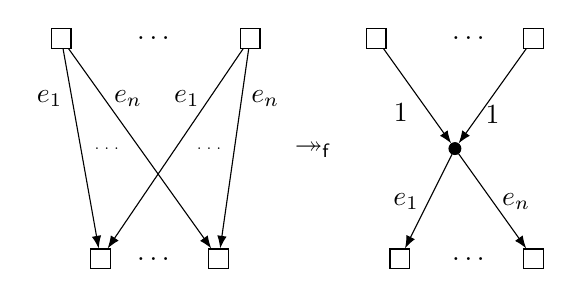
\begin{tikzpicture}[scale=1.0, every node/.style={transform shape}]
            % Left side (before)

            \begin{scope}[shift={(-.5,0)}]
          %  \node[] (p1) at (0.5,0.5) {$p_1$};
            \node[state] (p1) at (0.5,0) {};
               \node[state] (pn) at (2.9,0) {};
            \node[state] (q1) at (1,-2.8) {};
            \node[state] (q2) at (2.5,-2.8) {};
            \node (dots) at (1.7,-2.8) {$\dots$};
            \node (dots) at (1.7,0) {$\dots$};
            \node (ad) at (1.1,-1.4) {\tiny $\dots$};
            \node (ad) at (2.4,-1.4) {\tiny $\dots$};
            \draw[arr] (p1) to node[left, near start] {$e_1$} (q1);
            \draw[arr] (p1) to node[right, near start] {$e_n$} (q2);
            \draw[arr] (pn) to node[left, near start] {$e_1$} (q1);
            \draw[arr] (pn) to node[right, near start] {$e_n$} (q2);
            \end{scope}
            % Arrow between rules
            \node (i) at (3.2,-1.4) {$\twoheadrightarrow_{\mathsf{f}}$};
           % \node[below=1.4cm of i] {Factorization};

            % Right side (after)
            % \pgfmathsetmacro{\shift}{.5}
            \begin{scope}[shift={(3.5,0)}]
                \node[state] (sp1) at (.5,0) {};
                \node[state] (spn) at (2.5,0) {};
                \node[state] (sq1) at (0.8,-2.8) {};
                \node[state] (sq2) at (2.5,-2.8) {};
                \node[circ] (c) at (1.5,-1.4) {};
                \node (sdots) at (1.7,-2.8) {$\dots$};
            \node (sdots) at (1.7,0) {$\dots$};
            \draw[arr] (c) to node[left] {$e_1$} (sq1);
            \draw[arr] (c) to node[right] {$e_n$} (sq2);
            \draw[arr] (sp1) to node[left, yshift=-6pt, midway ] {$1$} (c);
            \draw[arr] (spn) to node[right, below ] {$1$} (c);
            \end{scope}
        \end{tikzpicture}\\[25pt]
          \textbf{Unproductivity elimination}  & &\textbf{Factorization} \\[20pt]
            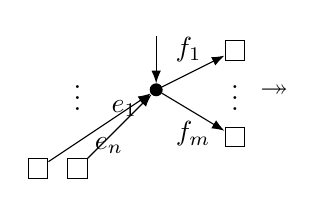
\begin{tikzpicture}[node distance=1.8cm, scale=1.0, every node/.style={transform shape}]
            % Left side (before)
            \node[circ] (c) at (0,0) {};
            \draw[arr] ([yshift=6mm]c.north) -- node[left,lab] {} (c.north);  
               \node[state] (q1) at (-1,-1) {}; 
            \node (q) at (-1,0) {$\vdots$};  
            \node[state] (qn) at (-1.5,-1) {};
            \node[state] (p1) at (1,.5) {};  
            \node (p) at (1,0) {$\vdots$};  
            \node[state] (pn) at (1,-.6) {};      
            \draw[arr] (c) to node[above] {$f_1\ $} (p1);
            \draw[arr] (c) to node[below, midway] {$\tiny{f_m}$} (pn);
            \draw[arr] (q1) to node[above, midway] {$\ e_1$} (c);
            \draw[arr] (qn) to node[below, midway] {$\ \ e_n $} (c);
            % Arrow between rules
            \node (i) at (1.5,0) {$\twoheadrightarrow$};
            %\node[below=1.2cm of i] {Zero rule};
            % Right side (after)
        \end{tikzpicture}&&           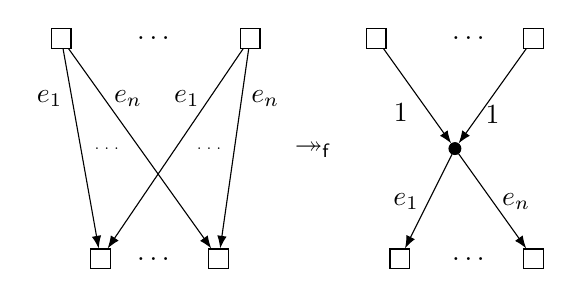
\begin{tikzpicture}[scale=1.0, every node/.style={transform shape}]
            % Left side (before)

            \begin{scope}[shift={(-.5,0)}]
          %  \node[] (p1) at (0.5,0.5) {$p_1$};
            \node[state] (p1) at (0.5,0) {};
               \node[state] (pn) at (2.9,0) {};
            \node[state] (q1) at (1,-2.8) {};
            \node[state] (q2) at (2.5,-2.8) {};
            \node (dots) at (1.7,-2.8) {$\dots$};
            \node (dots) at (1.7,0) {$\dots$};
            \node (ad) at (1.1,-1.4) {\tiny $\dots$};
            \node (ad) at (2.4,-1.4) {\tiny $\dots$};
            \draw[arr] (p1) to node[left, near start] {$e_1$} (q1);
            \draw[arr] (p1) to node[right, near start] {$e_n$} (q2);
            \draw[arr] (pn) to node[left, near start] {$e_1$} (q1);
            \draw[arr] (pn) to node[right, near start] {$e_n$} (q2);
            \end{scope}
            % Arrow between rules
            \node (i) at (3.2,-1.4) {$\twoheadrightarrow_{\mathsf{f}}$};
           % \node[below=1.4cm of i] {Factorization};

            % Right side (after)
            % \pgfmathsetmacro{\shift}{.5}
            \begin{scope}[shift={(3.5,0)}]
                \node[state] (sp1) at (.5,0) {};
                \node[state] (spn) at (2.5,0) {};
                \node[state] (sq1) at (0.8,-2.8) {};
                \node[state] (sq2) at (2.5,-2.8) {};
                \node[circ] (c) at (1.5,-1.4) {};
                \node (sdots) at (1.7,-2.8) {$\dots$};
            \node (sdots) at (1.7,0) {$\dots$};
            \draw[arr] (c) to node[left] {$e_1$} (sq1);
            \draw[arr] (c) to node[right] {$e_n$} (sq2);
            \draw[arr] (sp1) to node[left, yshift=-6pt, midway ] {$1$} (c);
            \draw[arr] (spn) to node[right, below ] {$1$} (c);
            \end{scope}
        \end{tikzpicture}\\
\end{tabular}
%}
\end{center}~\\[15pt]
\caption{\label{fig:rewriting-rules} Rewriting rules for networks}
     \end{figure}

%      As in other rewriting systems, such as state elimination for automata, 
% we require that initial and final states have no incoming 
% and no outgoing transitions, respectively. 
% We introduce a \emph{normalization} operation that enforces that.

  

% \begin{definition} Let $C$ be a network with initial state list $(I_1, \ldots, I_n)$.
% The \emph{normalization} of~$C$, denoted~$\norm{C}$, is the network obtained as follows: 
% \begin{itemize}
%     \item Add a list of fresh states $(J_1, \ldots, J_n)$ forming the new initial state list.  
%     \item Add a $1$-transition from $J_i$ to $I_i$, for each $i\in \{1,\ldots,n\}$.
%     \item Add a fresh state, called the \emph{sink}, which becomes the unique final state.
%     \item For each former final state, add a $1$-transition to the sink.
% \end{itemize}
% \end{definition}





\begin{definition} 
Let $\varphi$ be a function from a finite set $S$ to regular expressions. The \emph{network} $\mathcal{N}(\varphi)$ is defined as follows.
Its set of states is $S$ plus a fresh state $f$. Its set of initial states is $S$ and its unique final state is $f$. For every $s \in S$, there is a transition $(s, \varphi(s), f)$.
\end{definition}




\begin{definition}
Let $N$ be a network. If there is a function $\varphi$ from the set of initial states of $N$ to regular expressions, such that  ${N} \twoheadrightarrow^* \mathcal{N}(\varphi)$, we say that $N$ \emph{reduces} to $\varphi$ and write:
\[N \twoheadrightarrow^* \varphi.\]
\end{definition}

\begin{remark}
  When $N$ is a chart, and thus $\varphi$ can be identified with a single expression $e$, in that case, we write:
  \[N \twoheadrightarrow^* e.\] 
  \end{remark}

\begin{definition}
A regular expression is \emph{star-safe} if every sub-expression $f^*$ satisfies $f\Uparrow$.
\end{definition}


\begin{proposition}
  Every expression is provably equivalent to a star-safe one.
    ~\label{prop:every-expression-is-equivalent-to-a-safe-one}
\end{proposition}

\begin{proposition} For every star-safe expression $e$, $\milner{e}$ reduces to $e$.
    ~\label{prop:Milner-is-reducible}
\end{proposition}


\begin{lemma} Let $M$ and $N$ be two rooted charts. We have:
  $$\begin{array}{rcl}
    M\twoheadrightarrow^* e\ \text{and}\ N\twoheadrightarrow^* f & \Longrightarrow&  (M+N) \twoheadrightarrow^* (e+f)\ \text{ and }\ (M \cdot N) \twoheadrightarrow^* (e \cdot f)\\[6pt]
    M \Uparrow\ \text{and}\ M \twoheadrightarrow^* e & \Longrightarrow&  M^* \twoheadrightarrow^* e^*.
  \end{array}$$
\end{lemma}

\section{Labeling Charts}

\begin{definition} Let $N$ be a network with a transition relation  $\Delta$. A \emph{labeling} of $N$ is a function
$\ell:Q \mapsto Re(\Sigma)$ satisfying, for every state $p$:
\[\ell(p) \ \equiv \underset{(p,a, q) \in \Delta}{\sum} a \ell(q) + \chi(p)\]
The restriction of $\ell$ to the set of initial states of $N$ is called the \emph{interface} of the labeling. If $N$ admits a labeling with interface $\varphi$, we write \[N\models \varphi.\]
\end{definition}




The rewriting rules interact well with the notion of labelability. Indeed, labelability is preserved by the inverse of the reduction relation, and as a corollary we deduce that reducibility implies labelability (Section~\ref{sec:reducible-implies-decorable}).  Labelability is also preserved under reduction (under a safety hypothesis), and a corollary of this is a form of confluence (Section~\ref{sec:confluence-of-rewriting-system}).

 \subsection{Reducible implies labelable}\label{sec:reducible-implies-decorable}
   \begin{lemma}
     Let $M$ and $N$ be two networks and $\varphi$ a function. We have:
     \[ M\twoheadrightarrow N \ \text{ and }\ N \models \varphi \quad \Longrightarrow \quad M \models \varphi. \]
      \end{lemma}
      \begin{proof}
        By case analysis on the applied rewriting rule.
      \end{proof}

     By noticing that for every finite domain function $\varphi$, we have
     $\mathcal{N}(\varphi)\models \varphi$, we obtain the following proposition.
 \begin{proposition}
    For every network $N$ and function $\varphi$, we have:
    \[ N\twoheadrightarrow^* \varphi \quad \Longrightarrow \quad N \models \varphi.\]~\label{prop:reducible-implies-decorable}~\\[-25pt]
 \end{proposition}


% \begin{corollary} For every expression $e$, $\milner{e}\models e$.~\label{prop:milner-chart-is-decorable}
% ~\label{prop:Milner-is-decorable}\end{corollary}



\subsection{Confluence of the rewriting system}\label{sec:confluence-of-rewriting-system}

  \begin{definition} Let $N$ be a network over regular expressions.
 A cycle in $N$ is \emph{final} if all its transition labels are final. We say that $N$ is \emph{safe for reduction} if it has no final cycles.
 \end{definition}

 \begin{remark} Note that charts over the alphabet $\Sigma$ are safe for reduction.
 \end{remark}

 
  \begin{lemma} Let $M$ and $N$ be networks safe for reduction and let $\varphi$ be  a function. We have:
    \[  N \models \varphi  \ \text{ and }\  N \twoheadrightarrow M\quad \Longrightarrow\quad M \models \varphi.\] ~\label{lem:stable-by-red}
  \end{lemma}
\begin{proof}
  By case analysis on the rewriting rule.
\end{proof}


\begin{proposition} Let $N$ be a network safe for reduction and let $\varphi$ and $\psi$ be two functions. We have:
 \[ N \models \varphi\ \text{ and }\  N\twoheadrightarrow^* \psi\quad \Longrightarrow\quad \varphi\equiv \psi.\] 
\end{proposition}
\begin{proof} 
By iterating lemma~\ref{lem:stable-by-red}, and noticing that:
 \[\mathcal{N}(\psi)\models \varphi\quad \Rightarrow \quad \varphi\equiv \psi.\]\vspace{-10pt}
\end{proof}

As a consequence, we show a sort of confluence for the rewriting system.
\begin{corollary} Let $N$ be a network. We have: 
  \[ N \twoheadrightarrow^* \varphi\ \text{ and }\  N\twoheadrightarrow^* \psi\quad \Longrightarrow\quad \varphi\equiv \psi.\]
  for every functions $\varphi$ and $\psi$. 
  \label{cor:confluence}
\end{corollary}




\section{Adding, removing and duplicating initial states}

Promoting states to initial states, or conversely removing their initial-state status, does not change a network's reducibility. Likewise, duplicating an initial state does not change it either.

\begin{proposition} Let $N$ be a network and $\varphi$ be a function such that:
  \[N\twoheadrightarrow^* \varphi.\]
  Let $M$ be the network obtained from $N$ by restricting its set of initial states, while all other data remain identical.. If $\psi$ is the restriction of $\varphi$ to the initial states of $M$, then:
  \[  M \twoheadrightarrow^* \psi.\] 
\end{proposition}

\begin{proposition} 
  Let $N$ be a network and $\varphi$ be a function such that:
  \[N\twoheadrightarrow^* \varphi.\]
  Let $M$ be the network obtained from $N$ by extending its set of initial states, while all other data remain identical. There is an extension $\psi$ of $\varphi$ such that:
  \[  M \twoheadrightarrow^* \psi.\] 
\end{proposition}

\begin{proposition} Let $N$ be a network and $\varphi$ be a function such that:
  \[N\twoheadrightarrow^* \varphi.\]
  Let $i$ be an initial state of $N$ and let $M$ be the network obtained from $N$ by adding a fresh initial state $j$ with no ingoing transitions and the same outgoing transitions as $i$.  There is an extension $\psi$ of $\varphi$ such that:
  \[  M \twoheadrightarrow^* \psi\quad \text{ and }\quad \psi(i) = \psi(j).\] 
\end{proposition}






\section{Chart quotients}

\subsection{Definition and properties of quotients}
\begin{definition}
  The quotient of a chart $M$, denoted $\quotient{M}$, is the chart obtained from $M$ by identifying all bisimilar states.
\end{definition}

\begin{proposition}~\label{prop:quotient-preserves-labelability} For every chart $M$ and expression $e$, we have:
  \[\quotient{M}\models e\quad \Longrightarrow\quad M\models e.\]
\end{proposition}
In the remainder of this section, we show that the quotient of a Milner chart is reducible.

\begin{proposition}For every expression $e$, $\quotient{M(e)}$ is reducible.~\label{prop:quotient-of-Milner-chart-is-labelable}
\end{proposition}


\subsection{Traps}

\begin{definition} A \emph{trap} in a chart is a set of states closed under transitions: if a state is in the trap, then all its successors are also in the trap.

  The \emph{frontier} of a trap is the set of states outside the trap which are either: $i)$ final or $ii)$ have an outgoing transition to a state in the trap.

  A \emph{summary} of a trap is a function whose domain is the frontier of the trap.
\end{definition}



\begin{definition}
Let $C$ be a chart, $T$ a trap of $C$, and $\varphi$ a summary of $T$.

We denote by $C[T,\varphi]$ the chart obtained as follows.  
First, all states belonging to the trap~$T$ are removed.  
Then, for each state $q$ on the frontier, we create a fresh copy of $q$, we declare this copy final, we make $q$ non-final if it was, and we add a transition from $q$ to its copy labelled by~$\varphi(q)$.  
All other states and transitions remain unchanged.

A \emph{trap abstraction} of $C$ is a chart of the form $C[T,\varphi]$ for some trap $T$ of $C$ and some summary $\varphi$ of $T$.
\end{definition}

\begin{example} Example of a trap abstraction.
\end{example}

\begin{proposition} A trap abstraction of a Milner chart is a Milner chart.
\end{proposition}

\section{Proof of completeness}



We can now prove the completeness of Milner's axiomatization.

\begin{theorem} For every expressions $e$ and $f$, we have:
  $$ e\sim f \quad \Longrightarrow \quad e\equiv f.$$
\end{theorem}
\begin{proof}
 Let $e$ and $f$ be two expressions such that $e\sim f$. The charts $M(e)$ and $M(f)$ being trim and bisimilar, they have the same quotient $Q$.  By Proposition~\ref{prop:quotient-of-Milner-chart-is-labelable}, there is an expression $g$ such that: $$Q\models g.$$
 Using Proposition~\ref{prop:quotient-preserves-labelability}, we have:
   $$M(e)\models g\quad \text{ and } \quad M(f)\models g.$$
  By Proposition~\ref{prop:milner-chart-is-decorable}, we also  have:
   $$M(e)\models e\quad \text{ and } \quad M(f)\models f$$
  By Corollary~\ref{cor:confluence}, we have then:
   $$e\equiv g\quad \text{ and } \quad f \equiv g.$$Hence $e\equiv f$.
\end{proof}



\section{Erasing transitions from Milner charts}

In general, erasing transitions from a Milner chart does not yield a Milner Chart. However, we show that if the erased transitions are \emph{coherent} and \emph{border}, then it does.

\begin{definition} Let $M$ be a chart whose transition set is $\Delta$.~\\[-5pt]

  A transition of $M$ is \emph{border} if its source is either initial or final.~\\[-5pt]
  
  A set $\Gamma\subseteq \Delta$ is \emph{coherent}, if for every  transitions  
  $t, u\in \Delta$, whose sources are final and having the same label and target, we have:\vspace{-4pt}
   $$ t\in \Gamma \quad \Leftrightarrow \quad u\in \Gamma.$$ 
\end{definition}


\begin{definition}  
A \emph{letter erasing} of an expression $e$ is an expression obtained from $e$ by replacing some letter occurrences by $0$.
\end{definition}

\begin{proposition} Let $e$ be an expression and $\Gamma$ be a coherent set of border transitions of $M(e)$. There is a letter erasing $f$ of $e$ such that:
  $$ M(e)\setminus \Gamma = M(f).$$
\end{proposition}



  \begin{thebibliography}{9}
\bibitem{Antimirov1996}
V. Antimirov, ``Partial derivatives of regular expressions and finite automaton constructions,'' \emph{Theoretical Computer Science}, 155(2): 291--319, 1996.
\end{thebibliography}

\end{document}

\subsection{Charts with bisimilar roots are bisimilar}

\begin{proposition} Let $M$ and $N$ be charts and $e$ and $f$ expressions. We have:
  $$ M\models e,\ \ N\models f \ \text{ and }\ e\sim f \quad \Longrightarrow\quad M\sim N.$$
\end{proposition}
\begin{proof} let $\ell$ and $\ell'$ be labelings of $M$ and $N$ with roots $e$ and $f$ respectively.  We show that the relation $R$ between the states of $M$ and $N$ defined as follows:
  $$ (p,q)\in R \quad \Leftrightarrow \quad \ell(p) \sim \ell'(q), $$
  is a bisimulation between $M$ and $N$.
\end{proof}
If a chart has a labeling with root $e$, then it is bisimilar to $M(e)$.
\begin{corollary} For every chart $M$ and expression $e$, we have:
  $$M\models e \quad \Longrightarrow\quad M\sim M(e).$$ 
\end{corollary}